\documentclass[]{book}

%These tell TeX which packages to use.
\usepackage{array,epsfig}
\usepackage{amsmath}
\usepackage{amsfonts}
\usepackage{amssymb}
\usepackage{amsxtra}
\usepackage{amsthm}
\usepackage{mathrsfs}
\usepackage{color}
\usepackage[margin=2cm,top=2.5cm,headheight=16pt,headsep=0.1in,heightrounded]{geometry}
\usepackage{fancyhdr}
\pagestyle{fancy}
\usepackage{tikz}


%Here I define some theorem styles and shortcut commands for symbols I use often
\theoremstyle{definition}
\newtheorem{defn}{Definition}
\newtheorem{thm}{Theorem}
\newtheorem{cor}{Corollary}
\newtheorem*{rmk}{Remark}
\newtheorem{lem}{Lemma}
\newtheorem*{joke}{Joke}
\newtheorem{ex}{Example}
\newtheorem*{soln}{Solution}
\newtheorem{prop}{Proposition}

\newcommand{\lra}{\longrightarrow}
\newcommand{\ra}{\rightarrow}
\newcommand{\surj}{\twoheadrightarrow}
\newcommand{\graph}{\mathrm{graph}}
\newcommand{\bb}[1]{\mathbb{#1}}
\newcommand{\Z}{\bb{Z}}
\newcommand{\Q}{\bb{Q}}
\newcommand{\R}{\bb{R}}
\newcommand{\E}{\bb{E}}
\newcommand{\C}{\bb{C}}
\newcommand{\N}{\bb{N}}
\newcommand{\M}{\mathbf{M}}
\newcommand{\m}{\mathbf{m}}
\newcommand{\MM}{\mathscr{M}}
\newcommand{\HH}{\mathscr{H}}
\newcommand{\Om}{\Omega}
\newcommand{\Ho}{\in\HH(\Om)}
\newcommand{\bd}{\partial}
\newcommand{\del}{\partial}
\newcommand{\bardel}{\overline\partial}
\newcommand{\textdf}[1]{\textbf{\textsf{#1}}\index{#1}}
\newcommand{\img}{\mathrm{img}}
\newcommand{\ip}[2]{\left\langle{#1},{#2}\right\rangle}
\newcommand{\inter}[1]{\mathrm{int}{#1}}
\newcommand{\exter}[1]{\mathrm{ext}{#1}}
\newcommand{\cl}[1]{\mathrm{cl}{#1}}
\newcommand{\ds}{\displaystyle}
\newcommand{\vol}{\mathrm{vol}}
\newcommand{\cnt}{\mathrm{ct}}
\newcommand{\osc}{\mathrm{osc}}
\newcommand{\LL}{\mathbf{L}}
\newcommand{\UU}{\mathbf{U}}
\newcommand{\support}{\mathrm{support}}
\newcommand{\AND}{\;\wedge\;}
\newcommand{\OR}{\;\vee\;} 
\newcommand{\Oset}{\varnothing}
\newcommand{\st}{\ni}
\newcommand{\wh}{\widehat}
\newcommand{\vect}[1]{\overrightarrow{#1}}

%Pagination stuff.
%\setlength{\oddsidemargin}{0in}
%\setlength{\evensidemargin}{0in}
\setlength{\textheight}{9.in}
\setlength{\textwidth}{6.5in}
\cfoot{page \thepage}
\lhead{MEU302 - Alg\`ebre}
\rhead{Interro 3}
\pagestyle{fancy}


\begin{document}

\subsection*{Rappel de cours}

\newpage
\subsection*{Exercice 1}
\subsection*{Exercice 1.1}
On a 
$$e^A = \sum_{n= 0 \to \infty}{\frac{1}{k!}A^k} = A^0 + A^1 + \frac{1}{2}A^2 + \frac{1}{6}A^3 + \ldots + \frac{1}{n!}A^n + \ldots$$

On a aussi
$$
A^p = 
\begin{bmatrix}
\lambda_1^p & 0 & \ldots & 0 \\    
0 & \lambda_2^p  & \ddots & 0 \\
\vdots & \ddots & \ddots & 0 \\    
0 & \ldots & 0 & \lambda_n^p\\
\end{bmatrix}
$$

Donc 
$$
e^A = A^0 + A^1 + \frac{1}{2}A^2 + \frac{1}{6}A^3 + \ldots + \frac{1}{n!}A^n + \ldots
$$
$$= 
\begin{bmatrix}
    \lambda_1^0 & 0 & \ldots & 0 \\    
    0 & \lambda_2^0  & \ddots & 0 \\
    \vdots & \ddots & \ddots & 0 \\    
    0 & \ldots & 0 & \lambda_n^0\\
\end{bmatrix}
+
\begin{bmatrix}
    \lambda_1^1 & 0 & \ldots & 0 \\    
    0 & \lambda_2^1  & \ddots & 0 \\
    \vdots & \ddots & \ddots & 0 \\    
    0 & \ldots & 0 & \lambda_n^1\\
\end{bmatrix}
+
\frac{1}{2}
\begin{bmatrix}
    \lambda_1^2 & 0 & \ldots & 0 \\    
    0 & \lambda_2^2  & \ddots & 0 \\
    \vdots & \ddots & \ddots & 0 \\    
    0 & \ldots & 0 & \lambda_n^2\\
\end{bmatrix}
+
\ldots
+
\frac{1}{p!}
\begin{bmatrix}
    \lambda_1^p & 0 & \ldots & 0 \\    
    0 & \lambda_2^p  & \ddots & 0 \\
    \vdots & \ddots & \ddots & 0 \\    
    0 & \ldots & 0 & \lambda_n^p\\
\end{bmatrix}
+\ldots    
$$
$$
= 
\begin{bmatrix}
    1 + \lambda_1 + \frac{1}{2}\lambda_1^2 + \ldots + \frac{1}{p!}\lambda_1^p + \ldots & 0 & \ldots & 0 \\    
    0 & \lambda_2 + \frac{1}{2}\lambda_2^2 + \ldots + \frac{1}{p!}\lambda_2^p + \ldots  & \ddots & 0 \\
    \vdots & \ddots & \ddots & 0 \\    
    0 & \ldots & 0 & \lambda_n + \frac{1}{2}\lambda_n^2 + \ldots + \frac{1}{p!}\lambda_n^p + \ldots\\
\end{bmatrix}
$$

Le d\'eveloppement limit\'e de $e^x = x^0 + x^1 + \frac{1}{2}x^2 + \ldots + \frac{1}{p!}x^p + \ldots$

Donc
$$
e^A = 
\begin{bmatrix}
    e^\lambda_1 & 0 & \ldots & 0 \\    
    0 & e^\lambda_2  & \ddots & 0 \\
    \vdots & \ddots & \ddots & 0 \\    
    0 & \ldots & 0 & e^\lambda_n\\
\end{bmatrix}   
$$

Si la matrice $A$ est diagonalisable alors $\exists P et D, A = PDP^{-1}$. Donc on a $A^n = A.A. \ldots . A = PDP^{-1}.PDP^{-1}.\ldots.PDP^{-1} = PD^nP^{-1}$. Donc
$$
e^A = \sum_{k = 0 \to \infty}{\frac{1}{k!}A^k} = \sum_{k = 0 \to \infty}{\frac{1}{k!}PD^kP^{-1}} = P.\sum_{k = 0 \to \infty}{\frac{1}{k!}D^k}.P^{-1} = P.e^D.P^{-1}
$$
On peut sortir les 2 matrices $P$ et $P^{-1}$ de la somme car elles peuvent \^etre vues comme des constantes dans la somme (ind\'ependence par rapport a $n$).

\subsection*{Exercice 1.2}
Si la matrice $A$ est nilpotente alors $\exists n, A^n = 0$ Donc
$$
e^A = \sum_{k = 0 \to \infty}{\frac{1}{k!}A^k} = \sum_{k = 0 \to n-1}{\frac{1}{k!}A^k} + \sum_{k = n \to \infty}{\frac{1}{k!}A^k} = \sum_{k = 0 \to n-1}{\frac{1}{k!}A^k} + \frac{1}{n!}.0 + \frac{1}{n+1!}.0 + \ldots =  \sum_{k = 0 \to n-1}{\frac{1}{k!}A^k}
$$

Soit un polynome $P \in \R[X]$ de degr\'es $n$ alors 
$$
P(A) = a_0 A^0 + a_1 A^1 + a_2 A^2 + \ldots + a_n A^n = \sum_{k=0 \to n}{a_k A^k}
$$
D\'efinissons le polynome $P$ tel que $\forall k \in \N^{*}, a_k = \frac{1}{k!}$ et $a_0 = 1$
donc 
$$
P(A) = \sum_{k=0 \to n}{a_k A^k} = a_0 A^0 + \sum_{k=1 \to n}{\frac{1}{k!} A^k} = \sum_{k=0 \to n}{\frac{1}{k!} A^k}= e^A
$$
si la matrice $A$ est nilpotente de rang $n+1$. 

\subsection*{Exercice 1.3}
On a $A = D+N$ avec $D$ une matrice diagonale, $N$ une matrice nilpotente et $DN = ND$. Donc
$$
e^A = \sum_{k = 0 \to \infty}{\frac{1}{k!}A^k} = \sum_{k = 0 \to \infty}{\frac{1}{k!}(D+N)^k}
$$ 

$$
e^De^N = \sum_{k = 0 \to \infty}{\frac{1}{k!}D^k} . \sum_{l = 0 \to n-1}{\frac{1}{l!}N^l}
$$
Comme $N$ est nilpotente de rang $n$ on a 
$$
\sum_{k = 0 \to \infty}{\frac{1}{k!}D^k} . \sum_{l = 0 \to \infty}{\frac{1}{l!}N^l}
$$
Donc
$$
= D^0\sum_{l = 0 \to \infty}{\frac{N^{l}}{l!}} + D^1\sum_{l = 0 \to \infty}{\frac{N^{l}}{l!}} + \frac{1}{2}D^2\sum_{l = 0 \to \infty}{\frac{N^{l}}{l!}} \ldots +  \frac{1}{n!}D^n\sum_{l = 0 \to \infty}{\frac{N^{l}}{l!}} + \ldots
$$
$$
= \sum_{l = 0 \to \infty}{D^0\frac{N^{l}}{l!}} + \sum_{l = 0 \to \infty}{D^1\frac{N^{l}}{l!}} + \sum_{l = 0 \to \infty}{\frac{1}{2}D^2\frac{N^{l}}{l!}} \ldots +  \sum_{l = 0 \to \infty}{\frac{1}{n!}D^n\frac{N^{l}}{l!}} + \ldots
$$
$$
= \sum_{k = 0 \to \infty}\sum_{l = 0 \to \infty}{\frac{D^k}{k!}\frac{N^{l}}{l!}}
$$

$$
= \sum_{m = 0 \to \infty}\sum_{k = 0 \to m}{\frac{D^k}{k!}\frac{N^{m-k}}{(m-k)!}}
$$
$$
= \sum_{m = 0 \to \infty}\frac{1}{m!}\sum_{k = 0 \to m}{\frac{m!}{k!(m-k)!}D^kN^{m-k}}
$$
Comme les matrices $N$ et $D$ commuttent,
$$
= \sum_{m = 0 \to \infty}{\frac{1}{m!}(D+N)^m} = e^{D+N}
$$

On peux faire le m\^eme raisonnement en partant de $e^Ne^D$

Pas besoin de $D$ diagonale??

\subsection*{Exercice 1.4}
D'apr\`es le Th\'eor\`eme de la d\'ecomposition de Dunford, toute matrice $M$ peut de d\'ecomposer en une somme de deux matrices $D$ et $N$ tel que $D$ soit diagonalisable, $N$ soit nilpotente et les 2 matrices commuttent ($ND = ND$).
Donc pour calculer, on trouver les matrices $A$ et $B$ et $e^M= e^{A+B} = e^Ae^B$. Comme $A$ est diagonalisable on a $A=PDP^{-1}$. Donc $e^A = Pe^DP^{-1}$. La matrice $D$ est diagonale donc le calcul de $e^D$ est trivial (question 1). COmme $B$ est nilpotente de rang $n$, on peut faire le calcul de $e^B$ car on a une borne $n$.

\subsection*{Exercice 2}
\subsection*{Exercice 2.1}
Exercice 12.3.

Montrons que si $F_1$ et $F_2$ sont deux sous espace affines de $E$ alors $F_1 \subset F2 \implies F_1 \cup F_2$ est un sous-espace affine. On a $F_1 \subset F2 \implies F_1 \cup F_2 = F_2$ et $F_2$ est un sous espace affine par hypoth\`ese donc $F_1 \cup F_2$ l'est \'egalement. M\^eme raisonnement pour $F_2 \subset F1 \implies F_1 \cup F_2$ est un sous-espace affine.

Montrons que si $F_1$ et $F_2$ sont deux sous espace affines de $E$ alors si $F_1 \cup F_2$ est un sous-espace affine alors $F_1 \subset F2$ ou $F_2 \subset F1$. Preuve par l'absurde. Il existe $P$ tel que $P \in F_1 - F_2$ et $Q$ tel que $Q \in F_2 - F_1$. On a $P \in F_1 \in F_1 \cup F_2$ et $Q \in F_2 \in F_1 \cup F_2$. Donc $P-Q \in F_1 \cup F_2$.
On peut \'ecrire $P = Q + (P-Q)$ donc $(P-Q) \not \subset F_2$ car sinon $P$ serait dans $F_2$ et contredirait l'hypoth\`ese $P \in F_1 - F_2$. De m\^eme, $Q = P + (Q-P)$ donc $(Q-P) \not \subset F_1$ car sinon $Q$ serait dans $F_1$ et contredirait l'hypoth\`ese $Q \in F_2 - F_1$. Par cons\'equent $P-Q \not \subset F_1 \cup F_2$ ce qui contredit notre hypoth\`ese de d\'epart.


Exercice 13.1

On a $a \in V$ donc $a = u_1 + k_a \overrightarrow{V}$, de m\^eme $b \in W$ donc $b = u_2 + k_b \overrightarrow{W}$. par d\'efinition $vect<a,b> = a - b = u_1 + k_a \overrightarrow{V} -u_2 - k_b \overrightarrow{W}$ ou $u_1 - u_2 = vect<a,b> - k_a \overrightarrow{V} + k_b \overrightarrow{W}$

On a $c \in T$ donc $c = u_1 + k_c \overrightarrow{T} = u_2 + k'_c \overrightarrow{T}$. donc $u_1-u_2 = (k'c-k_c) \overrightarrow{T}$.

En regroupant les 2 on a $(k'c-k_c) \overrightarrow{T} = vect<a,b> - k_a \overrightarrow{V} + k_b \overrightarrow{W}$

\subsection*{Exercice 3}
\subsection*{Exercice 3.1}
$E= \{ (x^2 + y^2 = 1)\}$. C'est l'\'equation param\'etrique du cercle de centre $(0,0)$ et de rayon 1.

\begin{tikzpicture}[scale=2]
    \draw[help lines, color=gray!80, dashed] (-1.5,-1.5) grid (1.5,1.5);
    \draw[->] (-1.5,0) -- (1.5,0) node[right] {$x(t)$};
    \draw[->] (0,-1.5) -- (0,1.5) node[above] {$y(t)$};
             
    \draw[thick,variable=\t,domain=0:360,samples=200]
       plot ({cos(\t)},{sin(\t))});
\end{tikzpicture}

Pas un espace affine (ni une droite, ni un point ni un plan)

\subsection*{Exercice 3.2}
$E= \{ ((x-1)^2 + 0(y-1)^2 = 0)\}$, il faut que $x=1$ et $y$ quelconque donc $E$ est la droite verticale passant par le point $(1,0)$.
\begin{tikzpicture}[scale=2]
    \draw[help lines, color=gray!80, dashed] (-1.5,-3.5) grid (1.5,3.5);
    \draw[->] (-1,0) -- (1.5,0) node[right] {$x(t)$};
    \draw[->] (0,-3) -- (0,3) node[above] {$y(t)$};
             
    \draw[thick,variable=\t,domain=-3:3,samples=20]
       plot ({1},{\t});
\end{tikzpicture}

Espace affine $\begin{bmatrix} 1 \\ 0 \end{bmatrix} + (\R \begin{bmatrix} 0 \\ 1 \end{bmatrix})$.

\subsection*{Exercice 3.3}
$E= \{ ((x-1)^2 + (y-1)^2 = 4)\}$, C'est l'\'equation param\'etrique du cercle de centre $(1,1)$ et de rayon 2.

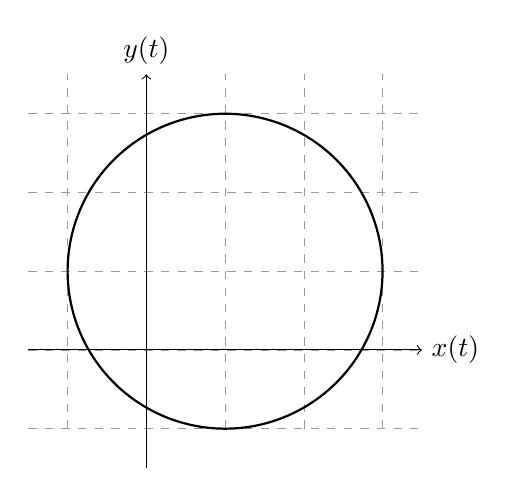
\begin{tikzpicture}[scale=1]
    \draw[help lines, color=gray!80, dashed] (-1.5,-1) grid (3.5,3.5);
    \draw[->] (-1.5,0) -- (3.5,0) node[right] {$x(t)$};
    \draw[->] (0,-1.5) -- (0,3.5) node[above] {$y(t)$};
             
    \draw[thick,variable=\t,domain=0:360,samples=200]
       plot ({2*cos(\t)+1},{2*sin(\t)+1});
\end{tikzpicture}

Pas un espace affine (ni une droite, ni un point ni un plan)

\subsection*{Exercice 3.4}
$E= \{ ((x-2)^2 + (y-2)^2 = -1)\}$, pas de solution $E = \emptyset$.

Pas un espace affine (ni une droite, ni un point ni un plan)

\subsection*{Exercice 3.5}
$E= \{ ((x+1)^2 + (y-1)^2 = 0)\}$, solution est un seul point $(-1,1)$.

Espace affine $\begin{bmatrix} -1 \\ 1 \end{bmatrix} + (\R \begin{bmatrix} 0 \\ 0 \end{bmatrix})$.

\subsection*{Exercice 3.6}
$E= \{ (x+1)^2 - (y-1)^2 = 0)\} = \{ (x+1)^2 = (y-1)^2\} = \{ |x+1| = |y-1| = |1-y|\}$. Premi\`ere solution $x=-y$, seconde solution $y = x+2$. Donc 2 droites.

\begin{tikzpicture}[scale=2]
    \draw[help lines, color=gray!80, dashed] (-3.5,-2) grid (1.7,4);
    \draw[->] (-3.5,0) -- (1.7,0) node[right] {$x(t)$};
    \draw[->] (0,-2) -- (0,4) node[above] {$y(t)$};
             
    \draw[thick,variable=\x,domain=-3:1.5,samples=50]
       plot ({\x},{-\x});
    \draw[thick,variable=\x,domain=-3:1.5,samples=50]
       plot ({\x},{\x+2});
\end{tikzpicture}

Union de 2 sous-espaces affines:
\begin{itemize}
    \item $\begin{bmatrix} -1 \\ 1 \end{bmatrix} + (\R \begin{bmatrix} 1 \\ 1 \end{bmatrix})$.
    \item $\begin{bmatrix} -1 \\ 1 \end{bmatrix} + (\R \begin{bmatrix} -1 \\ 1 \end{bmatrix})$
\end{itemize}
Ce n'est pas un sous espace affine. Car la relation de Chasles n'est pas respect'e si on prend le premier vecteur sur la premi\`ere droite et le second sur la seconde.

\end{document}

